

    %Abstract
    %Introduction (motivation for your work)
    %Background (literature review, or related work)
    %Methods (design and implementation)
    %Results and discussion  (include plots & figures, and detailed analysis in comparison to baseline and the literature, if applicable)
    %Conclusion

%\documentclass{article}
\documentclass[11pt,a4paper, twocolumn]{article}
%\usepackage[hyperref]{eacl2021}
\usepackage{times}
\usepackage{latexsym}
\usepackage{graphicx}
\renewcommand{\UrlFont}{\ttfamily\small}
\usepackage[nomarkers,nolists]{endfloat}
\usepackage{tabu}

\usepackage{microtype}


\newcommand\BibTeX{B\textsc{ib}\TeX}

\title{Testing Genre Specific Models for Social Media Summarization}

\author{Trevor Johnson \\
  UC Berkeley  \\
  \texttt{trevorj@berkeley.edu} \\\And
  Andrew Beckerman \\
  UC Berkeley \\
  \texttt{abeckerman@berkeley.edu} \\}

\date{}

\begin{document}


\maketitle
\begin{abstract}

We present a method to produce abstractive summaries of informal social media text via neural abstractive summarization. We test a model that has achieved state of the art text summarization performance in the news domain and evaluate their performance in the social media domain.
In addition, we test models trained on specific genres against a general model trained on all genres. We take this opportunity to show that training a general model produces higher rouge scores than a training a genre specific model.

\end{abstract}

\section{Introduction}

Text summarization is important for faster consumption of articles and text, saving time, and still providing the reader with the gist of an article. Figuring out what is ‘important’ in text summarization is challenging because the answer is highly dependent on the domain of the text, the target audience, and the goal of the summary itself.

Most summarization research is focused on news articles. However, as social media popularity increases, and in turn the generation of informal text, the need to summarize informal text will become more demanding.

With this in mind, we used the Webis-TLDR-17 corpus (Völske et al., 2017), a social media dataset, for our text summarization modeling. This dataset provides a summarization corpus from the domain of social media, consisting of 3 million reddit posts alongside so-called TL;DR summaries meaning "too long; didn't read".  These TL;DR summaries are written by social media posters writing long posts in anticipation of readers not having the patience to read an entire post. This gives us a text and summary written by the same person.

In addition, we wanted to explore the significance of understanding the genre of a post as it relates to model performance. We trained 4 separate models on 4 'genres' ('advice/story', 'gaming', 'media/lifestyle/sports' and 'other') and an overall model trained on all genres to evaluate whether a genre specific model can outperform a general model. To categorize the observations into different genres we used the subreddit \footnote{Subreddits are a forum dedicated to a specific topic on the website Reddit e.g., gaming, basketball, politics} of a post as a proxy for the 'genre' of the post. We feel the usefulness for understanding the importance of a genre specific model could potentially extend beyond social media and be helpful in text summarization in many other domains including news articles.

We evaluate the model performance by using ROUGE (Lin, 2004) metrics and comparing the model to human generated summaries.

\begin{table}
\centering
\begin{tabular}{lrll}
\hline \textbf{Dataset} & \textbf{# docs (train/val/test)} & \textbf{avg. post length} & \textbf{avg. summary legnth} \\ \hline
%\textbf{} & textbf{} & \multicolumn{words}{sentences} & \multicolumn{words}{sentences} \\
Overall & x & x & x \\
Advice/Story & 15,000/1,000/1,000 & x & x \\
Gaming & 15,000/1,000/1,000 & 4 & 15 \\
Media/Lifestyle/Sports & 15,000/1,000/1,000 & 4 & 15 \\
Other & 15,000/1,000/1,000 & 5 & 14 \\
\hline
\end{tabular}
\caption{\label{font-table} Comparison of summarization datasets with respect to overall corpus size, size of training, validation, and
test set, and average post and summary word length}
\end{table}

\begin{table}
\centering
\begin{tabu} to \textwidth {lX[r]X[l]X[l]}
\hline \textbf{Dataset} & \textbf{# docs (train/val/test)} & \textbf{avg. post length} & \textbf{avg. summary legnth} \\ \hline
%\textbf{} & textbf{} & \multicolumn{words}{sentences} & \multicolumn{words}{sentences} \\
Overall & x & x & x \\
Advice/Story & 15,000/1,000/1,000 & x & x \\
Gaming & 15,000/1,000/1,000 & 4 & 15 \\
Media/Lifestyle/Sports & 15,000/1,000/1,000 & 4 & 15 \\
Other & 15,000/1,000/1,000 & 5 & 14 \\
\hline
\end{tabu}
\caption{\label{font-table} Comparison of summarization datasets with respect to overall corpus size, size of training, validation, and
test set, and average post and summary word length}
\end{table}


\section{Background}
\label{sec:length}

In 2018, a tldr challenge (Syed et al., 2018) was organized where participants submitted a model to do abstractive summarization on the Webis-TLDR-17 corpus dataset. 5 model submissions were evaluated. They found both transf-seq2seq and pseudo-self-attn models generated the highest-quality text, but especially the latter often lacked information (REWORD). The main metric they used to evaluate the models was ROUGE. 

More recently, it has been shown a BART-based model works best for the Reddit dataset (Chen, 2020). Chen found that the BART model performed well on this abstractive dataset because of its ability to generate factual summaries over other models. Given this, we wanted to test a BART model combined with genre specific training data to see if we could record even better results.




\\

\section{Methods and Data}

\subsection{Exploratory Data Analysis}

Before modeling, we performed exploratory data analysis to better understand the reddit data. 
The dataset consisted of 3.8 million observations, each containing the full reddit post, the "TLDR" or summary of the post, and the subreddit. 
First, we explored word counts in each reddit post and summary by splitting on white space. 
Word counts were heavily skewed right in both the posts and summaries with average lengths of 278 and 27 respectively. 
While there were some posts and summaries with well over 1,000 words, most had word counts in a much more digestable range. 
90\% of the posts contained between 42 and 795 words, and 90\% of the summaries containing between 3 and 75 words. 
Figure 1 (UPDATE) shows histograms for the distribution of the distinct and total word counts for the reddit posts and summaries in our dataset. 
Studying these distributions helped us determine further hyperparameters when fitting models. 


\begin{figure}
  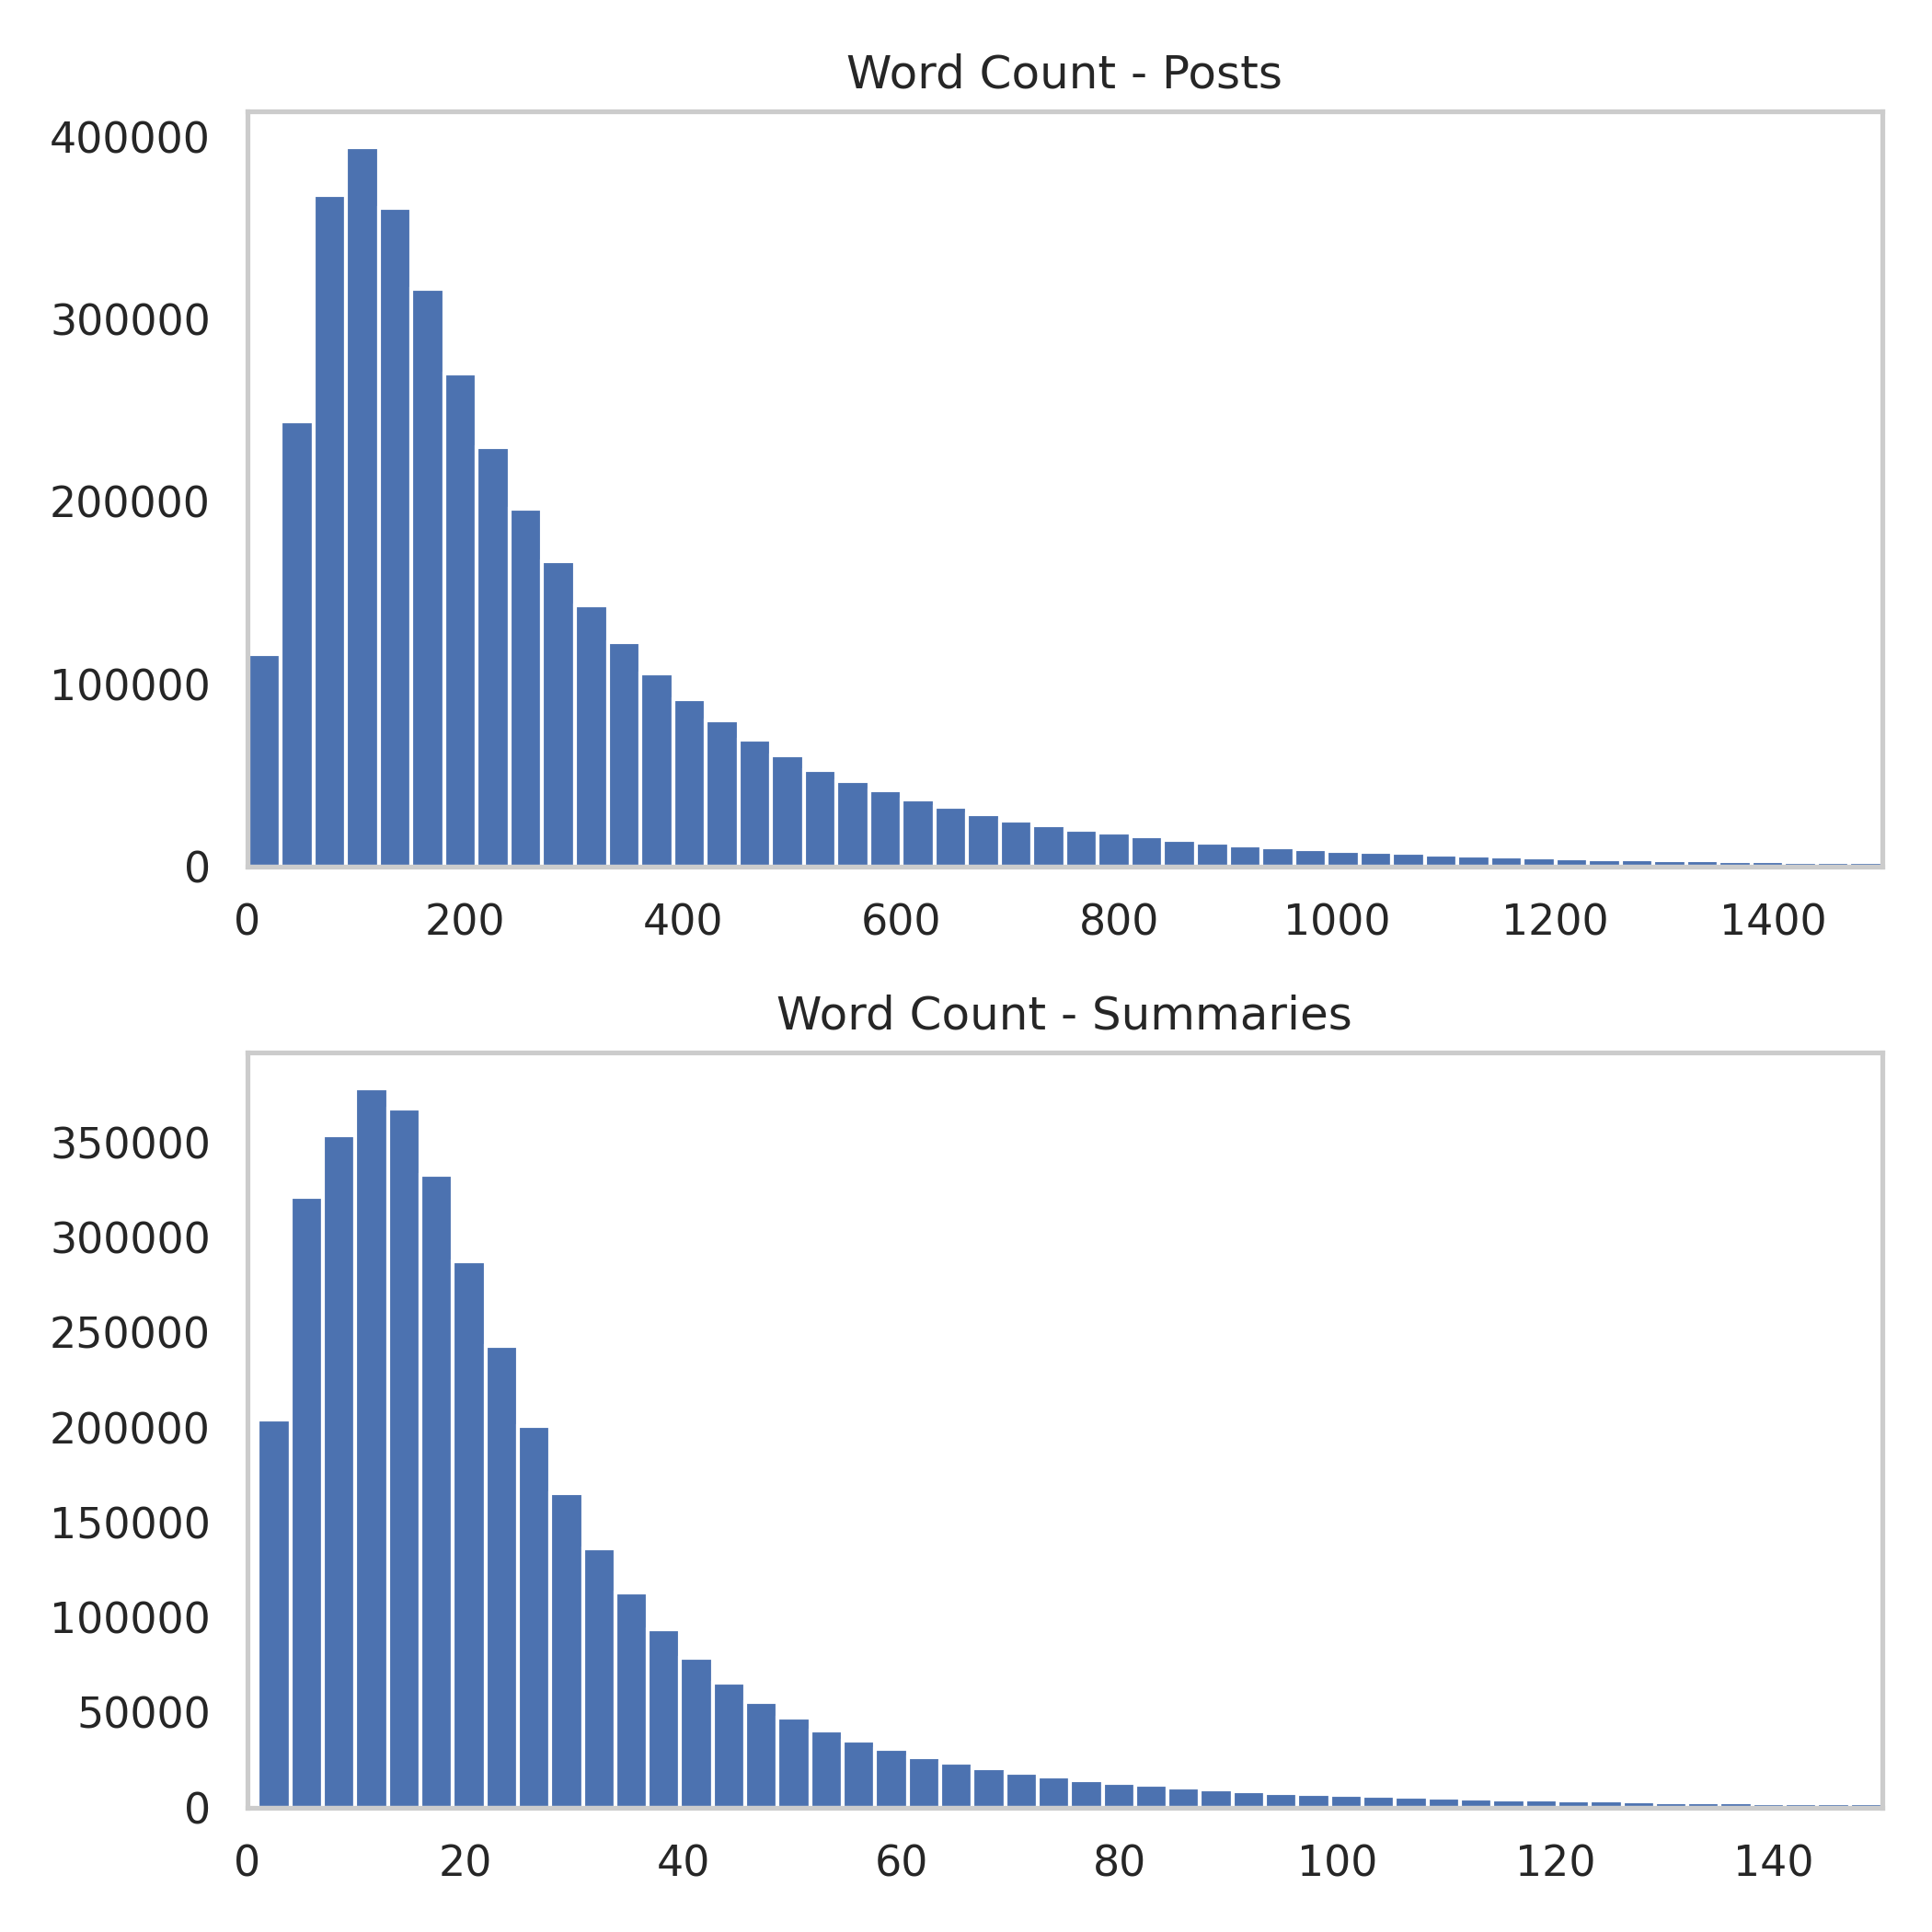
\includegraphics[width=\linewidth]{word_counts2.png}
  \caption{Word count distributions}
  \label{fig:word_counts}
\end{figure}

An initial investigation into the contents of the reddit posts and summaries showed that some contents nonsensically repeated 
the same word over and over, or would be extremely lengthy (over 3,000 words). 
With this in mind, we decided to filter down the dataset so it would only include reddit posts 
with word totals between 20 - 1000 and $\geq$ 10 unique words. 
In addition, each summary would only be between 2 - 100 total words and $\geq$ 2 unique words. 
With these filters in place, about 300,000 records were removed from our dataset. 


\subsection{Subreddit Genres}

Next, we explored the many subreddits in our dataset as we hoped to use this information to create segmented NLP models. 
Because there were over 28,000 distinct subreddits in our dataset, it would be unreasonable to build separate NLP models for every distinct subreddit. 
Thus, we sought to group these subreddits into more general genre categories. 


We considered creating a separate NLP model or use unsupervised learning techniques to systematically cluster the subreddits into similar categories, 
but doing so was outside of the scope of what we were seeking to learn. 
Thus, we ended up grouping the subreddits into genres by hand, making sure to categorize the most popular subreddits. 
In the end, we grouped the data into 4 distinct subreddit categories: gaming, advice/story, media/lifestyle/sports, and other. 
The counts for each subreddit genre can be found in figure 2. 

\begin{table}
  \centering
  \begin{tabular}{lrlll}
  \hline \textbf{Subreddit Genre} & \textbf{Post Count}\\ \hline
  Advice/Story & 1409813 \\
  Gaming & 501041 \\
  Media/Liftstyle/Sports & 455228 \\
  Other & 1184045 \\
  \hline
  \end{tabular}
  \caption{\label{font-table} Subreddit Genres}
\end{table}


\subsection{Modeling}

Sequence to sequence based transformer architectures have proven to achieve state of the art performance on the task of abstractive summarization.
In the original BART paper  (Lewis et al., 2019) (add link later: https://arxiv.org/pdf/1910.13461v1.pdf), the authors explain how BART performs 
particularly well at text generation as well as for comprehension tasks. Additionally, recent research has shown that by providing 
much more data to fine tune the BERT encoder, BART achieves state of the art performance on abstractive summarization tasks (Aghajanyan et al., 2020) (add link later: https://arxiv.org/pdf/2008.03156v1.pdf). 
Because of this strong recent performance and through initial exploration ourselves, we decided to use BART to 
generate abstractive summaries for our Reddit data. 

After we began experimenting with training BART models on our dataset and generating summaries, we quickly realized the scale of our dataset would be a problem. 
We frequently ran out of memory, or would exhaust compute times at both training and inference times. 
Thus, we decided to downsample our large dataset to a more reasonable scale for our project. 
From our cleaned dataset, we randomly sampled 17,000 observations from each of our 4 subreddit groups providing us with a total of 68,000 observations for our analysis. 

Through initial BART model exploration, we found that by using a BART model that was pretrained on both XSUM and CNN/DM datasets 
provided fluent abstractive summaries of our data. Thus, we decided to fine tune this model further to produce more faithful 
abstractive summaries. 

Because the Reddit posts often had very different content in the subreddit genres we generated, we hypothesized that by training 
separate BART models on each subreddit genre, we would maximize Rouge scores. Our analysis compares Rouge metrics from the following three models:

\begin{enumerate}
  \item BART Baseline: Pretrained on XSUM and CNN/DM without any fine tuning
  \item BART Full: Fine tuned on our entire Reddit dataset irrespective of subreddit
  \item BART Subreddit Split: Four separate models fine tuned on each of our four subreddit genre categories
\end{enumerate}

For each BART model, we tokenized the Reddit posts to a maximum of 1024 tokens, and the summaries to a maximum of 128 tokens. 
Doing so would adequately tokenize the entire text for over 97\% of our data, and avoid overburdening our BART model with tokens being too long. 

The baseline BART model was used to generate summaries on our 4,000 test dataset observations without any fine tuning.
We then trained a full BART model on our 60,000 observation training dataset irrespective of genre. 
Finally, the subredit split BART models were each trained on 15,000 training observations specific to a subreddit genre. 



\section{Results and discussion}

\subsection{Results}

After the fine tuning was completed, we used each of our three BART modeling approaches to generate abstractive summaries on 
our held out 4,000 test observations. Because over 90\% of our target summaries were shorter than 60 words, we decided to 
restrict our BART models to generate summaries with a maximum of 60 words. 

Our primary metric for evaluation was Rouge. 
Not only is Rouge the primary metric used to measure performance in related research, but the recall based approach 
was fitting for our analysis. Our 60 word maximum restriction provided a guardrail against the model having a terribly low precision, 
and we hoped our summaries would adequately use the same words found in the target summaries. 
Thus Rouge score felt appropriate to evaluate performance.
The resulting rouge scores for each modeling performance can be found in table X (UPDATE LATER).

\begin{table}
  \centering
  \begin{tabular}{lrlll}
  \hline \textbf{Test Set and Model} & \textbf{R-1} & \textbf{R-2} & \textbf{R-L} \\ \hline

  \multicolumn{4}{ l }{\emph{Genre: Advice/Story}} \\
  BART Baseline & 16.8 & 2.5 & 13.5 \\
  BART Full & 20.2 & 5.9 & 16.7 \\
  BART Subreddit Split & 20.0 & 5.7 & 16.4 \\
  \hline
  \multicolumn{4}{ l }{\emph{Genre: Media/Lifestyle/Sports}} \\
  BART Baseline & 14.8 & 2.1 & 12.1 \\
  BART Full & 14.3 & 3.5 & 12.2 \\
  BART Subreddit Split & 14.0 & 3.1 & 11.8 \\
  \hline
  \multicolumn{4}{ l }{\emph{Genre: Gaming}} \\
  BART Baseline & 15.3 & 1.9 & 12.0 \\
  BART Full & 16.5 & 4.1 & 13.5 \\
  BART Subreddit Split & 15.5 & 3.7 & 12.7 \\
  \hline
  \multicolumn{4}{ l }{\emph{Genre: Other}} \\
  BART Baseline & 14.9 & 2.0 & 12.1 \\
  BART Full & 16.6 & 4.0 & 13.9 \\
  BART Subreddit Split & 16.8 & 4.3 & 14.1 \\
  \hline

  \end{tabular}
  \caption{\label{font-table} ROUGE-1,2, and L scores for the generated summaries}
\end{table}

According to Rouge metrics, the full BART model generally outperformed the others. 
A key learning for us here is that in the case of our Reddit subset dataset, 
fine tuning on more data seems to be better than fine tuning on more specialized less data. 

\subsection{Error Analysis}

Next, we dug into the observations that had the lowest Rouge scores at inference time to study where our models went wrong. 
We were surprised to find that quite often, we felt our BART models produced TLDR summaries that were even better than the true target summaries. 
It seems the summaries that users generated were sometimes trying to be funny, or didn't actually summarize the content too well. 
Whereas our BART models seemed to do a better job. As an example, one post was a long story about a user's addiction to cannabis and his desire to 
abstain from smoking for a month. 
We've pasted the summaries below to show how we feel the BART summary does a better job summarizing the true and complete content.

\begin{itemize}
  \item True summary: Stay sober through October.
  \item BART Full summary: I'm taking a month off from smoking weed to prove to myself that it's not an issue.
\end{itemize}


On the other hand, there were some situations where our BART model clearly couldn't summarize the content very well. 
Sometimes the BART models would just return the first few words of the content and call that the summary. 

(FIND BAD EXAMPLE)

\subsection{Manual Summary Analysis}

Finally, as an additional benchmark for our models, we decided to manually generate summaries ourselves. 
We wrote 100 summaries, with 25 in each subreddit genre, and computed Rouge scores on them for comparison. 
While we recognize the small sample size results may not exactly extrapolate to the entire dataset, 
it gives a (idk rephrase later).
To keep the table simple, we've only compared the manual summaries to the full BART model below:

(UPDATE LATER)

Overall, it seems our manually generated summaries outperform the automatic BART models by several points. 
However, while generating the summaries, we found it particularly difficult to summarize the gamming subreddits. 
These posts often contains a lot of jargon that we didn't understand. 
The results above show that the BART model actually outperformed our manually generated summaries for this subreddit genre. 



\section{Conclusion}
We show a BART model trained on more data outperforms a model trained on a more specialized dataset with less data. 

Preliminary experiments showed when comparing the BART model's performance to a human generated summary, a human generated summary tended to receive a higher ROUGE score. 

\section*{References}
 \noindent Armen Aghajanyan; Akshat Shrivastava; Anchit Gupta; Naman Goyal; Luke Zettlemoyer; Sonal Gupta. 2021. Better Fine-Tuning by Reducing Representational Collapse. \emph{ArXiv: 2008.03156}
 \bigbreak
\noindent Chin-Yew Lin. 2004. Rouge: A package for auto-
matic evaluation of summaries. \emph{Text Summarization
Branches Out.}
\bigbreak
\noindent Mike Lewis; Yinhan Liu; Naman Goyal; Marjan Ghazvininejad; Abdelrahman Mohamed; Omer Levy; Veselin Stoyanov; Luke Zettlemoyer. 2020. BART: Denoising Sequence-to-Sequence Pre-training for Natural Language Generation, Translation, and Comprehension. \emph{ACL}
\bigbreak
\noindent Shahbaz Syed; Michael Völske; Nedim Lipka; Benno Stein; Hinrich Schütze; Martin Potthast. 2019. Towards summarization for social media-results of the tl;dr
challenge. \emph{In Proceedings of the 12th International Conference on Natural Language Generation, Tokyo, Japan, 29 October–1
November 2019; pp. 523–528}
\bigbreak
\noindent Yiran Chen; Pengfei Liu; Ming Zhong; Zi-Yi Dou; Danquing Wang; Xipeng Qiu; Xuanjing Huang. 2020. CDEvalSumm: An empirical study of cross-dataset evaluation
for neural summarization systems. \emph{"Findings of the Association for Computational Linguistics: EMNLP 2020"}

\end{document}

